\chapter{Nature-Inspired Algorithms: Detailed Study}
\section{Classification and shared search principles}
Metaheuristics guide search without a useful analytic optimum. Population methods maintain several candidates; trajectory methods modify one state. Exploration visits new regions, while exploitation refines promising ones.

\begin{figure}[htbp]\centering
\begin{tikzpicture}[node distance=7mm,box/.style={draw=Forest!35,rounded corners=3pt,fill=Soft,align=center,text width=31mm,minimum height=12mm,font=\small},arr/.style={-{Latex},Forest!50}]
\node[box,text width=56mm,fill=Forest,text=white] (root) {Metaheuristic search};
\node[box,below left=14mm and 34mm of root] (e) {Evolutionary\\GA, \textbf{DE}, ES};
\node[box,right=5mm of e] (s) {Swarm\\PSO, ACO, ABC};
\node[box,right=5mm of s] (p) {Physics-inspired\\SA, GSA};
\node[box,right=5mm of p] (o) {Other inspirations\\BBO, TLBO};
\draw[arr] (root)--(e);\draw[arr] (root)--(s);\draw[arr] (root)--(p);\draw[arr] (root)--(o);
\end{tikzpicture}
\caption{A teaching taxonomy. BBO is biogeography-inspired; categories overlap and do not rank algorithm quality.}
\end{figure}

GA combines selection and variation~\cite{holland1992adaptation}; PSO maintains individual and social memories~\cite{kennedy1995pso}. Ant System uses pheromone feedback~\cite{dorigo1996aco}; simulated annealing uses temperature-controlled acceptance~\cite{kirkpatrick1983annealing}.

\section{Representative update mechanisms}
A real-coded GA recombines selected parents, for example $\mathbf u=\alpha\mathbf x_a+(1-\alpha)\mathbf x_b$, then mutates and selects survivors. Our comparator uses tournament selection, blend crossover, Gaussian mutation, and elitism.

For PSO, particle velocity and position are updated as
\begin{align}
\mathbf v_i^{t+1}&=w\mathbf v_i^t+c_1\mathbf r_1\odot(\mathbf p_i-\mathbf x_i^t)+c_2\mathbf r_2\odot(\mathbf g-\mathbf x_i^t),\\
\mathbf x_i^{t+1}&=\mathbf x_i^t+\mathbf v_i^{t+1},
\end{align}
where $\mathbf p_i$ is the particle's best position and $\mathbf g$ the population best. In an ant system, transition preference is proportional to pheromone $\tau_{ij}^{\alpha}$ times heuristic desirability $\eta_{ij}^{\beta}$; pheromone is evaporated and reinforced by completed solutions~\cite{dorigo1996aco}. Simulated annealing accepts an uphill energy change $\Delta E$ with probability $\exp(-\Delta E/T)$, allowing controlled escape from local basins~\cite{kirkpatrick1983annealing}.

Firefly-style movement combines attraction and random perturbation, often expressed as $\mathbf x_i\leftarrow\mathbf x_i+\beta_0e^{-\gamma r_{ij}^2}(\mathbf x_j-\mathbf x_i)+\alpha\boldsymbol\epsilon$~\cite{yang2009firefly}. BBO models immigration and emigration between candidate habitats; a simple linear rate model uses $\lambda(s)=I(1-s/S)$ and $\mu(s)=Es/S$ for species count $s$~\cite{simon2008bbo}. ABC uses employed/onlooker/scout search roles~\cite{karaboga2007abc}; GWO models social hierarchy and hunting-inspired position updates~\cite{mirjalili2014gwo}. These are background methods, not additional CNN experiments.

\section{Differential Evolution in depth}
DE maintains $NP$ vectors in a normalized domain. In DE/rand/1, mutation for target $i$ is
\begin{equation}
\mathbf v_i=\mathbf x_{r_1}+F(\mathbf x_{r_2}-\mathbf x_{r_3}),\qquad r_1,r_2,r_3\ne i,
\end{equation}
with distinct donor indices. Difference vectors supply directions and scales informed by the current population~\cite{storn1997de,das2011survey}. The implementation freezes the donor population within each generation, so earlier evaluations do not change later donors in the same generation.

For a coordinate outside $[0,1]$, the repair rule draws a feasible value between the parent and the violated bound:
\begin{equation}
v_{ij}\leftarrow x_{ij}+r(b-x_{ij}),\quad r\sim U(0,1),\quad b\in\{0,1\}.
\end{equation}
Valid coordinates remain unchanged. This repair avoids repeated clipped boundary values but does not preserve uniform sampling.

Binomial crossover forms
\begin{equation}
u_{ij}=\begin{cases}v_{ij},&r_j<CR\ \text{or}\ j=j_{\mathrm{rand}},\\x_{ij},&\text{otherwise}.\end{cases}
\end{equation}
The forced coordinate ensures mutant contribution. Maximizing selection is
\begin{equation}
\mathbf x_i^{g+1}=\begin{cases}\mathbf u_i,&f(\mathbf u_i)\ge f(\mathbf x_i^g),\\\mathbf x_i^g,&\text{otherwise}.\end{cases}
\end{equation}
Best stored fitness is nondecreasing, although noisy fitness can misrepresent true quality. Difference-vector mutation is rotation-equivariant; coordinate-wise crossover prevents the whole algorithm from being rotation-invariant.

\begin{figure}[H]\centering
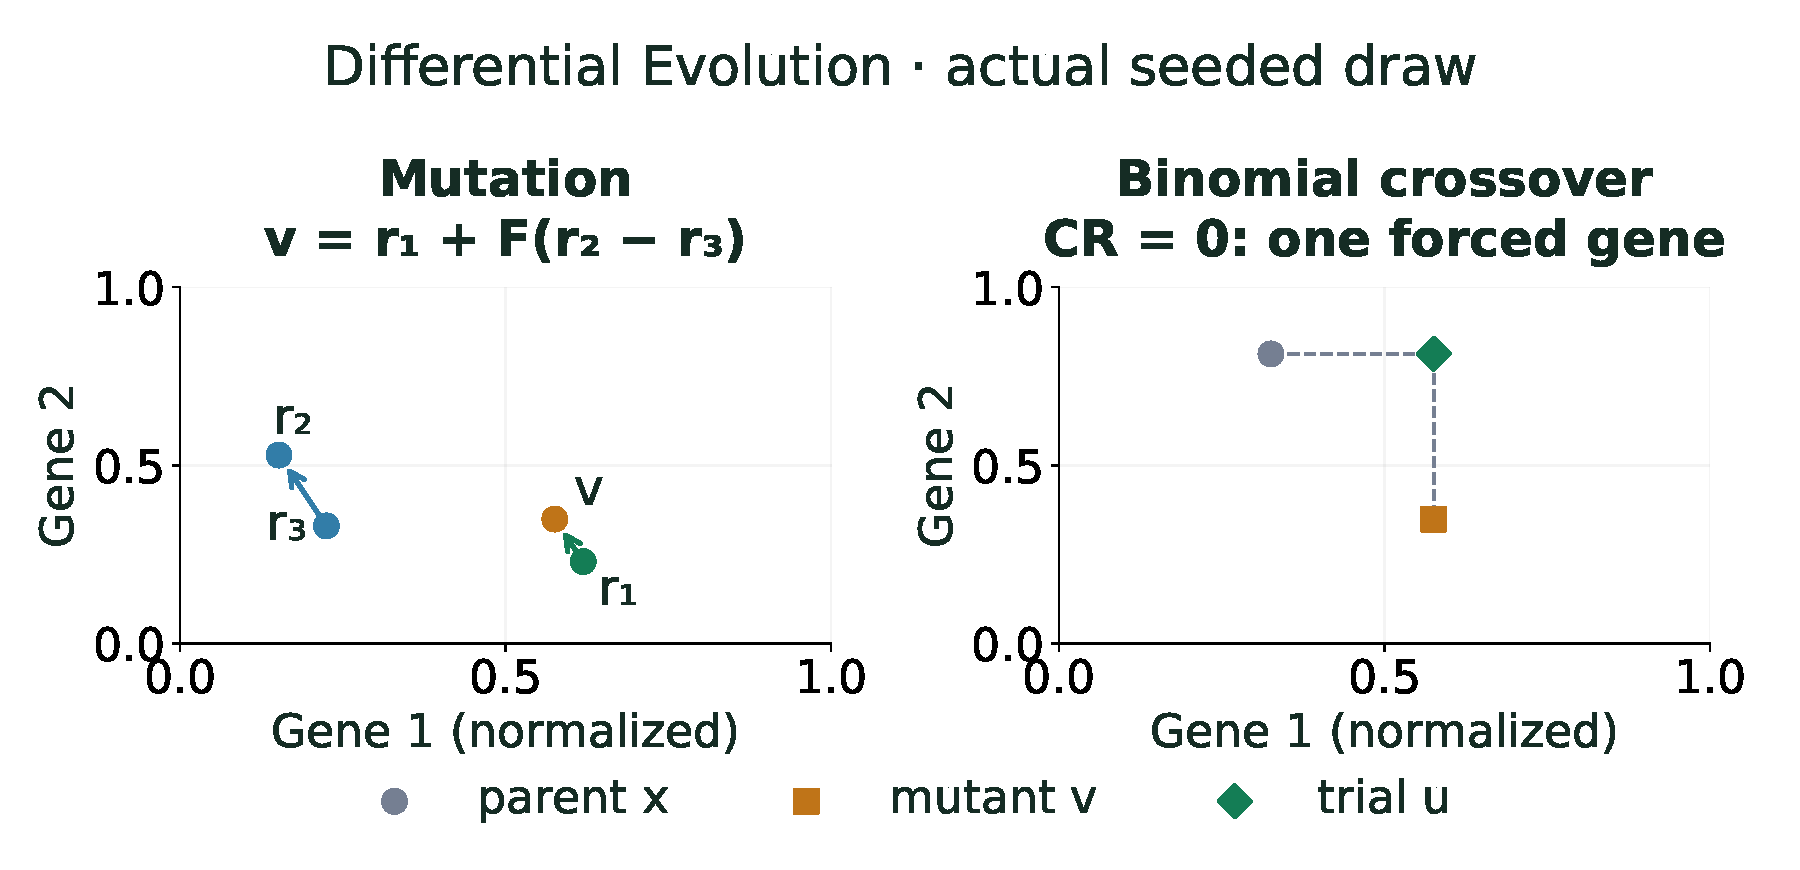
\includegraphics[width=.75\linewidth]{fig_de_operators_diagram.pdf}
\caption{Mutation, bound repair, and crossover using a recorded operator example.}\label{fig:deoperators}
\end{figure}

\section{Pseudocode and complexity}
\begin{algorithm}[H]
\caption{DE/rand/1/bin with deferred generation donors}
\begin{algorithmic}[1]
\Require Objective $f$, dimension $D$, population $NP$, generations $G$, $F$, $CR$
\State Initialize $X$ with Latin-hypercube samples in $[0,1]^D$
\State Evaluate all initial candidates and persist state
\For{$g=1,\ldots,G$}
\State $S\gets X$ \Comment{Frozen donor population}
\For{$i=1,\ldots,NP$}
\State Choose three distinct donor indices excluding $i$
\State $v\gets S_{r_1}+F(S_{r_2}-S_{r_3})$
\State Repair violating coordinates between $X_i$ and the bound
\State Form $u$ using binomial crossover and forced $j_{\mathrm{rand}}$
\State Evaluate $f(u)$ using the same fitness protocol
\If{$f(u)\ge f(X_i)$}\State $X_i\gets u$\EndIf
\State Atomically persist population, scores, and RNG state
\EndFor
\State Record fitness distribution, diversity, and success rate
\EndFor
\State \Return best recorded vector and full history
\end{algorithmic}
\end{algorithm}

The budget is $NP(G+1)$ including initialization; vector arithmetic is $O(GNP D)$, while training dominates time. Mean pairwise distance measures diversity, and replacement fraction measures success rate; both help identify stagnation.

\section{Variants and parameter control}
DE/best/1 uses the current best as its mutation base; DE/rand/2 uses two difference vectors; current-to-best strategies add attraction toward a leading vector. Such changes modify exploration and exploitation~\cite{das2016recent}. Increasing $F$ expands differential steps, while $CR$ changes coordinate mixing; their useful values depend on the landscape and available budget.

jDE retains successful individual control values~\cite{brest2006jde}; SHADE uses success histories and L-SHADE reduces population size~\cite{tanabe2013shade,tanabe2014lshade}. Only classic DE optimizes this CNN; adaptive variants are benchmark comparators.

\textbf{Why DE here.} Seven normalized genes support derivative-free mixed search with few controls and independent candidate evaluations. Noisy fitness, repeated recipes, and small populations limit coverage; equal-budget evidence determines usefulness~\cite{sorensen2015metaphors}.
